\documentclass[10pt]{article}

\usepackage{fullpage}
\usepackage{graphicx}
\usepackage{mathtools}
\usepackage{setspace}
\usepackage{mdwlist}
\onehalfspacing

\begin{document}
\title{Project Proposal\\Augmented Reality Image Processing System}
\author{Logan P. Williams \& Jos\'{e} E. Cruz Serrall\'{e}s}
\date{November 03, 2011}
\maketitle

\section{Abstract}
% should be revised, this is what we originally turned in 
In our project, we will implement an augmented reality system that can overlay a digital image on video of a real world environment. We begin by reading NTSC video from a video camera and storing it in ZBT SRAM. A picture frame with colored markers on the corners is held in front of the camera. We then perform chroma-based object recognition to locate the co-ordinates of the corners. Using these co-ordinates, we apply appropriate translation, scaling, rotation, and anti-aliasing FIR filters to fit the image to the boundary of the frame. If time allows, we will use a non-linear projective transformation to correct for perspective. We then output VGA video of the original captured image, with the processed image overlayed on top of the frame. The overlayed image (the ``augmentation'') can be arbitrary. When this image is the frame of video that was previously displayed, we call the system ``recursive'', as we obtain the same image contained within itself.
\newpage
\section{Top-Level Block Diagram}
\begin{figure}[h!]
\centering
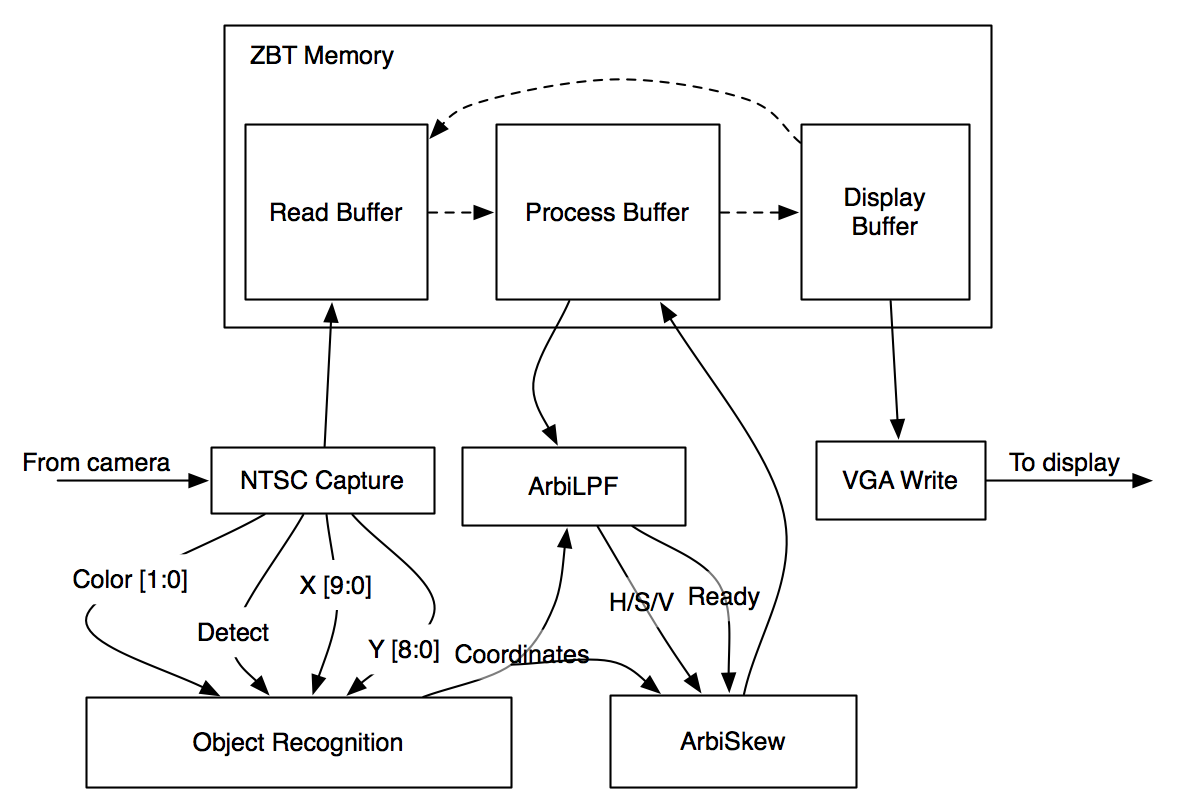
\includegraphics[width=0.7\textwidth]{block_diagram.png}
\caption{The block diagram of the augmented reality system}
\end{figure}
\section{Submodules}
% 1) inputs & outputs
% 2) some indication of its complexity and level of performance
%	a) number and type of arithmetic operations
%	b) size of internal memories
%	c) required throughput
%	etc.
% 3) how the module will be tested
% 4) who will be writing the module
\subsection{NTSC Capture (Logan)}
The NTSC capture module is almost unmodified from the code provided by 6.111. It takes as input an NTSC video signal, and writes pixels into ZBT Memory.

There are two modifications. The first allows the module to capture and store color data, converting it from Y/Cr/Cb to H/S/V. The second modification is added to support object recognition. When the Capture module sees a pixel of a hue that matches the target (blue, green, red, and yellow), it sends information (the color and its X/Y location) to the Object Recognition module.

\subsection{ZBT Memory (Jos\`{e})}
% Jose

\subsection{Object Recognition (Logan)}
The Object Recognition module collects ``interesting'' pixels located by the NTSC Capture module, and calculates the center of mass of each color, to find the location of the corners of the picture frame. It takes as input (1) the color of a detected pixel, (2) a flag that goes high for one clock cycle when a pixel is detected, (3) the X/Y coordinates of the pixel, and (4) a flag that goes high when the entire frame has been captured. It produces as output four sets of X/Y coordinates, one of the center of mass of each color.

The center of mass will be calculating with a simple linear weighting scheme, averaging the X and the Y coordinate for each pixel independently to find the center X/Y location, which are used by the ArbiLPF and the ArbiSkew module.

\subsection{ArbiLPF (Jos\`{e})}
% Jose
The inputs to ArbiLPF are (1) the previously displayed image and (2) the four coordinates of the dotted frame as detected from the NTSC output of the camera in the Object Recognition module. AbiLPF calculates the maximal amount by which the skewing algorithm will shrink the image, which will be referred to as M. ArbiLPF then applies a two-dimensional low-pass filter to the image, with a radial cutoff frequency of \( \frac{\pi}{M} \), in order to avoid aliasing in the ArbiSkew module.

Based on the downsampling factor M, the filter will select a set of coefficients from a lookup table and convolve the image values with these coefficients. This table of coefficients will correspond to the coefficients of two-dimensional extrapolations of one-dimensional FIR Parks-McClellan filters with cutoff frequencies of \( \frac{\pi}{M} \). Due to the limited number of multipliers on the FPGA, these two-dimensional filters will be constrained to have at most 144 coefficients, which constrains the one-dimensional filters to have at most 12 coefficients. Due to these constraints, the ripple and transition width specifications of the 1D filters will have to be lax. The radial symmetry of these 2D filters will be exploited to reduce the number of required multiplications by a factor of 4, to at most 36 multiplications per color per pixel.

\subsection{ArbiSkew (Logan)}
% Logan
The inputs to ArbiSkew are (1) the hue, saturation, and value of the last pixel produced by ArbiLPF, (2) a ready signal held high for one clock signal when ArbiLPF has processed a new pixel, and (3) the four coordinates of the corners of the frame provided by the Object Recognition module.

This function maps the original rectangular image to any convex quadrilateral, provided that all sides of the destination quadrilateral are shorter than the original, which is inherent in the overall system. A graphic representation of the transformation is shown in the figure below:

\begin{figure}[h!]
\centering
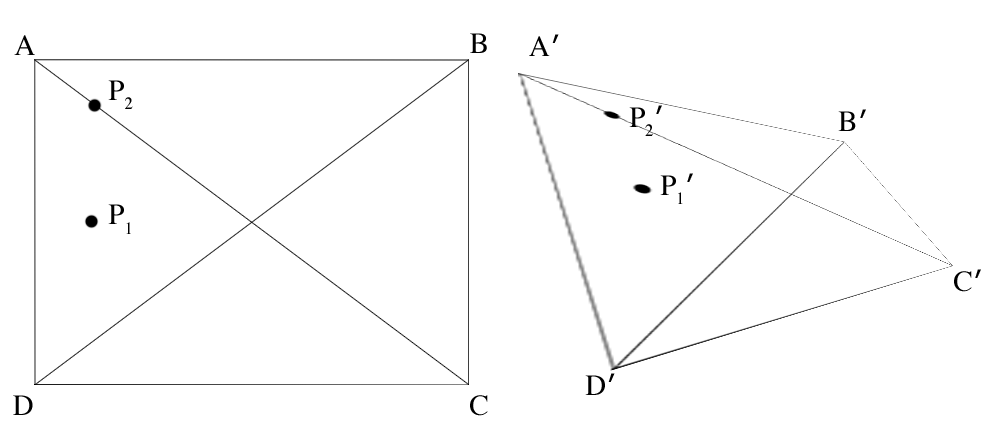
\includegraphics[width=0.65\textwidth]{arbiskew_graphic.png}
\caption{A visual representation of the result of the ArbiSkew module. Input is on the left, a possible output, for four coordinates $A\prime$, $B\prime$, $C\prime$, and $D\prime$ is on the right.}
\end{figure}

Mathematically, the algorithm works as follows:
\begin{enumerate*}
\item Calculate the distance of line $\overline{A\prime D\prime}$ and assign it to $d_{ad}$.
\item Do the same for $\overline{B\prime C\prime}$ and assign it to $d_{bc}$.
\item Create two ``iterator points," point $I_A$ and $I_B$ initially located at $A\prime$ and $B\prime$.
\item Let $o_x = 0$ and $o_y = 0$
\item Calculate the distance between the iterator points, assign it to $d_i$.
\item Create a third iterator point, $I_C$ at the location $I_A$.
\item Assign the pixel value of $I_C$ to pixel $(o_x, o_y)$ in the original image.
\item Move $I_C$ along line $\overline{I_A I_B}$ by an amount $= \frac{d_i}{width_{original}}$.
\item Increment $o_x$.
\item Repeat steps 7--9 until $I_C = I_B$.
\item Move $I_A$ along line $\overline{A\prime D\prime}$ by an amount $= \frac{d_{ad}}{height_{original}}$.
\item Move $I_B$ along line $\overline{B\prime C\prime}$ by an amount $= \frac{d_{bc}}{height_{original}}$.
\item Increment $o_y$.
\item Repeat steps 5--13 until $I_A = D\prime$ and $I_B = C\prime$.
\end{enumerate*}


This is feasible on the FPGA by using lookup tables to calculate $\sin$, $\cos$, and $\arctan$ for angle calculations. Besides that, it needs a relatively small number of multiplications, just two per pixel in the original image, and four per line in the original image. There is also a square root that is needed once per line, this can be implemented with either a look up table, or by using an iterative method of calculation.

\subsection{VGA Write}
% Jose

\section{External Components}
% Jose

\section{List of Goals}
% A calendar-like view of what deadlines we'll set ourselves, when everything should be operational, etc. Maybe this could be collapsed into the submodules section

\end{document}
